\documentclass{article}
\usepackage{amsfonts, amsmath, amssymb, amsthm} % Math notations imported
\usepackage{enumitem}
\usepackage{graphicx}
\usepackage{setspace}
\usepackage{indentfirst}
\usepackage[margin=1in]{geometry}
\graphicspath{{./images/}} % Path to images

% \begin{figure}[htb!]
%      \centering
%      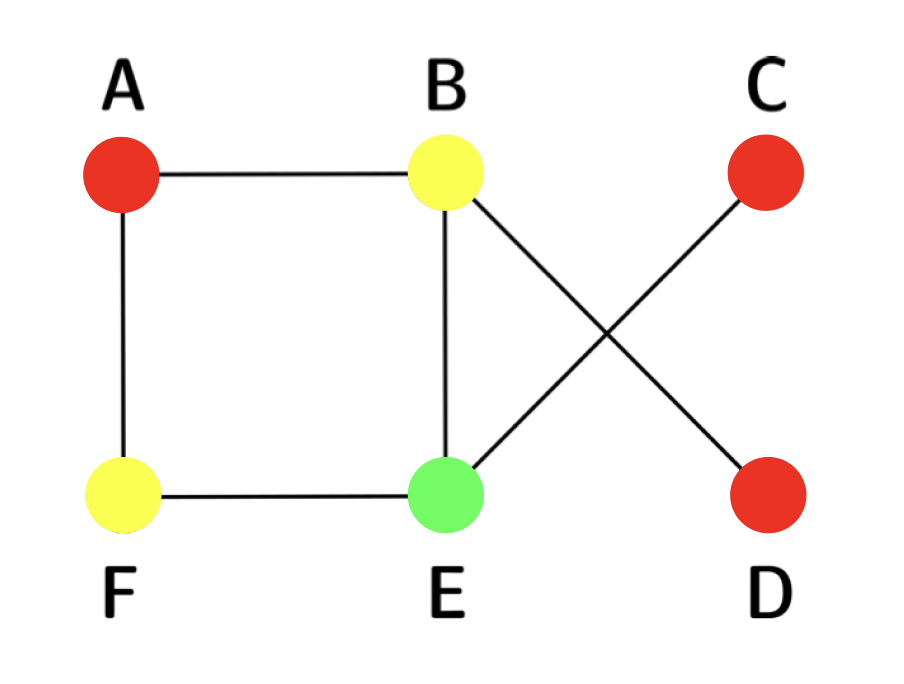
\includegraphics[scale=0.5]{coloring.png}
%      \caption{Coloring of the graph.}
% \end{figure}

% \begin{figure}[htb]
%     \qquad
%     \begin{minipage}{.4\textwidth}
%         \centering
%         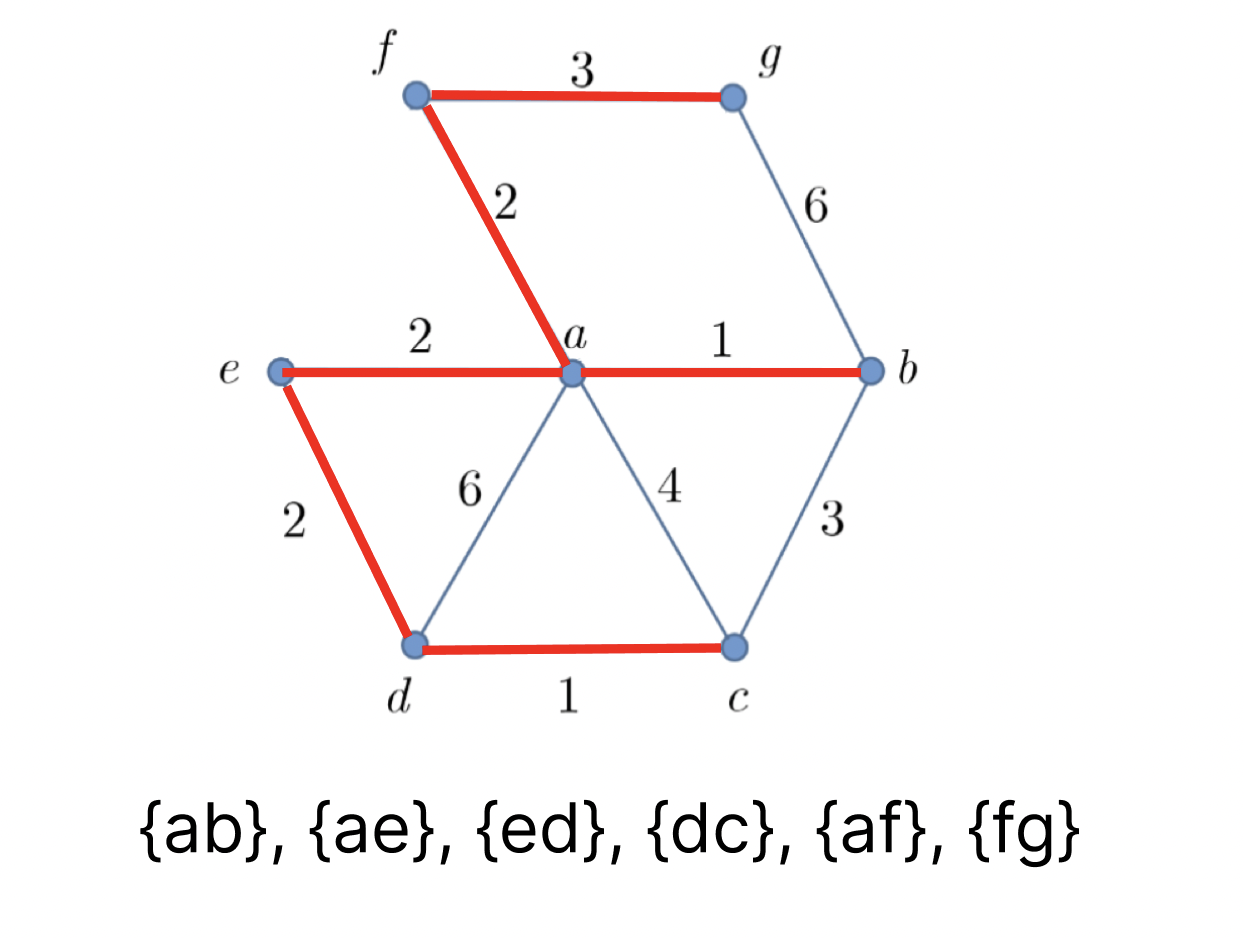
\includegraphics[scale=0.35]{prims.png}
%         \caption{}
%     \end{minipage}    
%     \qquad
%     \begin{minipage}{.4\textwidth}
%         \centering
%         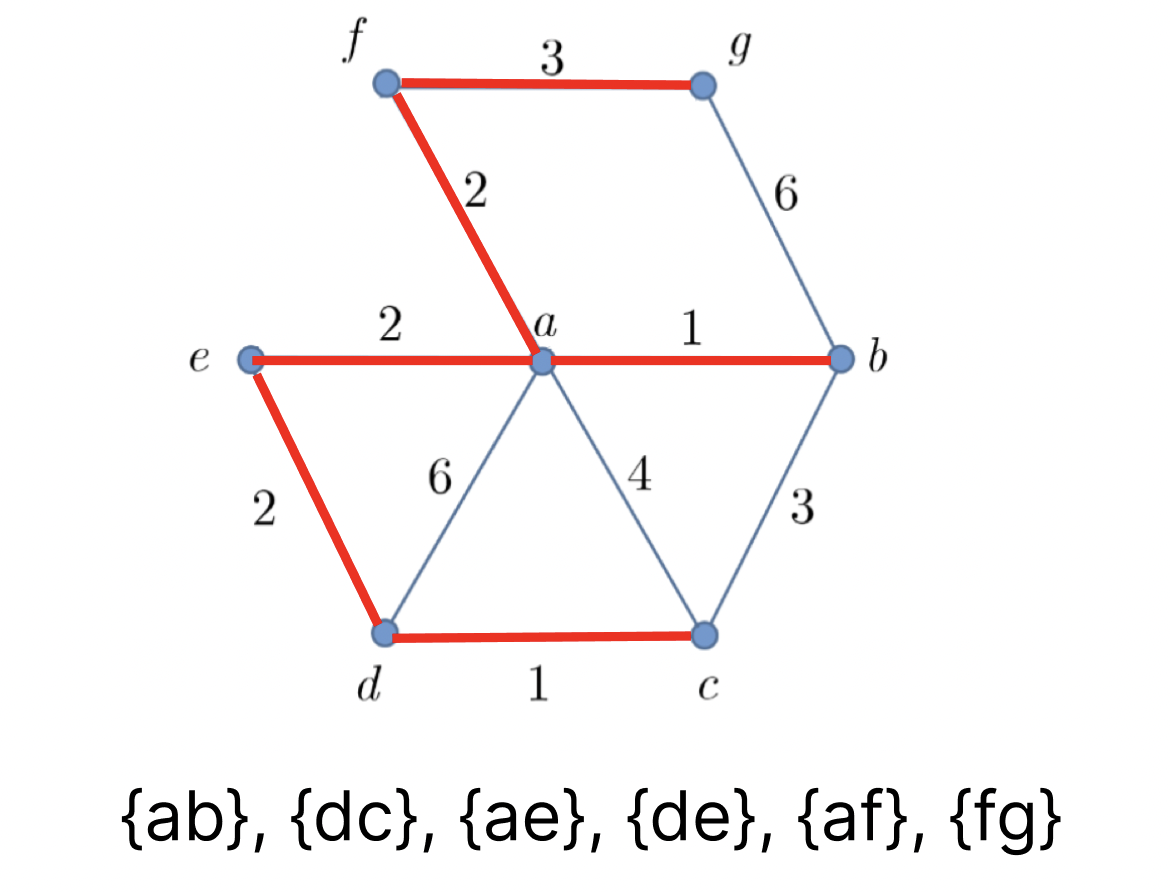
\includegraphics[scale=0.35]{kruskal.png}
%         \caption{}
%     \end{minipage}        
% \end{figure} 

\newtheorem{thm}{Theorem}
\newtheorem{proposition}[thm]{Proposition}
\newtheorem{cor}[thm]{Corollary}

% title information
\title{Math 110 HW7}
\author{Neo Lee}
\date{10/21/2023}

\setstretch{1.15}
% main content
\begin{document} 

% placing title information; comment out if using fancyhdr
\maketitle 

\subsection*{Problem 1.}
Suppose $V$ is finite-dimensional and $U$, $W$ are its subpaces. Prove that
$$ (U\cap W)^0 = U^0 + W^0.$$
\begin{proof}
    First we need the \emph{Lemma: $U^0 \cap W^0 = (U+W)^0$}.
    Consider $\phi \in U^0\cap W^0$ and $v = u+w \in U+W$, then 
    $$\phi(v) = \phi(u+w) = \phi(u) + \phi(w) = 0 + 0 = 0.$$
    Hence $\phi \in (U+W)^0$ and $U^0\cap W^0\subseteq (U+W)^0$.
    Now consider $\varphi \in (U+W)^0$, indeed for $u\in U$, $$\varphi(u) = \varphi(u+0) = 0,$$ and 
    for $w\in W$, $$\varphi(w) = \varphi(0+w) = 0$$ [notice $u+0$ and $0+w$ are both in $U+W$].
    Therefore, $\varphi \in U^0 \cap W^0$ and $(U+W)^0\subseteq U^0\cap W^0$. The \emph{Lemma} is 
    proved.

    \textbf{Now we back to the original problem.} Consider $\phi \in U^0+W^0$ and $v \in U\cap W$, then 
    $$\phi(v) = \varphi_u(v) + \varphi_w(v) =0+0=0 \qquad (\varphi_u\in U^0, \varphi_w\in W^0).$$
    Hence, $\phi\in (U+W)^0$ and $U^0+W^0\subseteq (U+W)^0$.

    Now consider the dimension of $(U\cap W)^0$ and $U^0 + W^0$.
    \begin{align*}
        \dim (U\cap W)^0 &= \dim V - \dim (U\cap W) \\
        &= \dim V - \dim U - \dim W + \dim (U+W) \\
        &= \dim V - (\dim V - \dim U^0) - (\dim V - \dim W^0) + (\dim V - \dim (U+W)^0) \\
        &= \dim U^0 + \dim W^0 - \dim (U+W)^0 \\
        &= \dim U^0 + \dim W^0 - \dim (U^0\cap W^0) \\
        &= \dim (U^0 + W^0).
    \end{align*}
    Since $U^0+W^0\subseteq (U+W)^0$ and $\dim (U^0 + W^0)=\dim (U\cap W)^0$, we have 
    $(U\cap W)^0 = U^0 + W^0$.
\end{proof}

\newpage
\subsection*{Problem 2.}
Suppose $V$ and $W$ are finite-dimensional, $T\in {\cal L}(V,W)$, and 
${\rm null}\, T' = {\rm span} (\varphi)$ for some $\varphi\in W'$. 
Prove that ${\rm range}\, T = {\rm null} \, \varphi$.  
Give an example of such a pair $T\neq 0$, $\varphi\neq 0$ for $V=\mathbb{R}^2$, $W=\mathbb{R}^3$.
\begin{proof}
    Notice $\mathrm{null} T' = (\mathrm{range} T)^0 = \mathrm{span}(\varphi)$. 
    Consider $w\in\mathrm{range}T$ and arbitrary $\lambda\in\mathbb{F}$, then 
    $$\lambda \varphi(w) = 0 \quad (\lambda\varphi \in (\mathrm{range}T)^0) \implies \varphi(w)=0.$$
    Hence, $\mathrm{range}T\subseteq\mathrm{null}\varphi$.

    Then we show that $\dim\mathrm{range}T=\dim\mathrm{null}\varphi$. For $\varphi\neq 0$,
    \begin{align}
        \dim \mathrm{range}T & = \dim W - \dim (\mathrm{range}T)^0 \nonumber \\
        & = \dim W - \dim \mathrm{span}(\varphi) \nonumber \\
        & = \dim W - 1 \nonumber \\
        & = \dim W - \dim \mathrm{range}\varphi \\
        & = \dim \mathrm{null}\varphi. \nonumber
    \end{align}
    (1) is true because $\varphi \neq 0$, so $\mathrm{range}\varphi =\mathbb{R}$.
    If $\varphi = 0$,
    \begin{align}
        \dim \mathrm{range}T & = \dim W - \dim (\mathrm{range}T)^0 \nonumber \\
        & = \dim W - \dim \mathrm{span}(\varphi) \nonumber \\
        & = \dim W - 0 \nonumber \\
        & = \dim \mathrm{null}\varphi. \nonumber
    \end{align}

    Since $\mathrm{range}T\subseteq\mathrm{null}\varphi$ and 
    $\dim\mathrm{range}T=\dim\mathrm{null}\varphi$, we have
    $\mathrm{range}T=\mathrm{null}\varphi$.

    \textbf{Example:} Let $T:(x,y)\mapsto (x,y,0)$ and $\varphi:(x,y,z)\mapsto z$. Then indeed, 
    $\mathrm{null}T'=\mathrm{span}(\varphi)$ [very obviously because $\varphi$ annihilates $\mathrm{range}T$], and 
    $$\mathrm{range}T=(x,y,0)=\mathrm{null}\varphi.$$
\end{proof}


\newpage
\subsection*{Problem 3.}
Let $p\in {\cal P}_n(\mathbb{C})$ for some $n$ and suppose there exist distinct real numbers 
$x_0$, $x_1$, $\ldots$, $x_n$ such that $p(x_j)\in \mathbb{R}$ for all $j=0, \ldots, n$. 
Prove that all coefficients of $p$ are real.
\begin{proof}
    \textbf{Lemma:} \emph{given distinct {\it data sites} $x_j$ 
    and arbitrary {\it data} $y_j$, $j=0,\ldots, n$, there is a unique polynomial  $p\in {\cal P}_n(\mathbb{R})$ 
    such that $p(x_j)=y_j$, for all $j=0,\ldots, n$.}

    We have shown in \textbf{Problem 4} that such unique polynomial takes the form 
    $$p(x)=\sum_{k=1}^{n}y_kL_k(x)\quad \text{for}\quad L_k(x)=\prod_{j=0,j\neq k}^{n}\frac{x-x_j}{x_k-x_j}.$$
    Then notice all the terms in this unique polynomial $p$ are real and expanding the product 
    $\prod_{j=0,j\neq k}^{n}\frac{x-x_j}{x_k-x_j}$ gives us a polynomial with real coefficients 
    [no imaginary parts can arise].
\end{proof}

\newpage
\subsection*{Problem 4.}
[Lagrange interpolation.] Prove {\it using linear algebra}: given distinct {\it data sites} $x_j$ 
and arbitrary {\it data} $y_j$, $j=0,\ldots, n$, there is a unique polynomial  $p\in {\cal P}_n(\mathbb{R})$ 
such that $p(x_j)=y_j$, for all $j=0,\ldots, n$. 
\begin{proof}
    Define the Lagrange basis polynomials 
    $$L_k(x)=\prod_{j=0,j\neq k}^{n}\frac{x-x_j}{x_k-x_j}.$$
    Notice each $L_k$ are of degree $n$ and hence each $L_k\in\mathcal{P}_n(\mathbb{R})$.
    Then notice these basis polynomials have the property that $L_k(x_k)=1$ and $L_k(x_j)=0$ for 
    $j\neq k$. 
    
    Then we can define 
    $$p(x)=\sum_{k=0}^{n}y_kL_k(x).$$
    Indeed, $p(x_j)=y_j$ because $L_j(x_j)=1$ and $y_jL_j(x_j)=y_j$ while $L_k(x_j)=0$ for $k\neq j$.
    To show that it's unique, assume to the contrary that there exists another polynomial
    $q\in\mathcal{P}_n(\mathbb{R})$ such that $q(x_j)=y_j$ for all $j=0,\ldots,n$. Then
    $$p(x)-q(x)=\sum_{k=0}^{n}y_kL_k(x)-q(x)=0.$$
    Notice $p(x)-q(x)$ is a polynomial of degree $n$ and has $n+1$ roots, which means 
    $p-q$ must be the zero polynomial because non-zero polynomial of degree $n$ has at most $n$ roots
    [Theorem 4.11].

    Therefore, $p-q=0\implies p=q$.

    \textbf{Alternative:} Define a linear map $T:\mathcal{P}_n(\mathbb{R})\to \mathbb{R}^{n+1}$ with 
    the action 
    $$T:p\mapsto (p(x_0), p(x_1), \cdots, p(x_n)).$$
    $T$ is indeed a linear map because 
    $$T(p+q) = ((p+q)(x_0), \cdots, (p+q)(x_n)) = (p(x_0), \cdots, p(x_n))+(q(x_0),\cdots, q(x_n))
    =T(p)+T(q)$$
    $$T(\lambda p) = (\lambda p(x_0),\cdots, \lambda p(x_n))=\lambda (p(x_0),\cdots, p(x_n))=
    \lambda T(p).$$
    
    Then notice $T$ is injective because for $T(p)=0$, $p$ must be zero when evaluated at distinct 
    data sites $\{x_j:j=[0,\dots,n]\}$, which means $p$ must have $n+1$ distinct roots.
    But an $n$ degree polynomial can only have at most $n$ distinct roots. Hence, $p$ must be the 
    zero polynomial and $\mathrm{null}T = \{0\}$. 
    
    Since $T$ is a linear map from $n+1$ dimension to $n+1$ dimension and is injective, it implies 
    $T$ is surjective. Therefore, there always exists a unique $p$ such that 
    $$T(p)=(p(x_0),\cdots,p(x_n))=(y_0, \cdots, y_n).$$
\end{proof}

\newpage
\subsection*{Problem 5.}
Prove that every polynomial of odd degree with real coefficients has a real zero.
\begin{proof}
    Assume for the sake of contradiction that there exists a polynomial of odd degree with real
    coefficients that has no real zero. Then we take the minimal example $p(x)$ with the 
    lowest degree. Notice $p$ can be factorized as follow 
    $$p(x)=(x-\lambda)(x-\bar{\lambda})q(x),$$
    where $\lambda$ is a complex zero of $p$ and $q(x)$ is a polynomial of degree $n-2$.
    Since we assumed $p$ to be the minimal example, $q(x)$ must have a real zero $x_0$.
    Then we have
    $$q(x)=(x-x_0)g(x)\implies p(x)=(x-\lambda)(x-\bar{\lambda})(x-x_0)g(x),$$
    which means $p$ has a real zero $x_0$ [contradiction].
\end{proof}

\end{document}
